\documentclass[10pt,a4paper]{article}
\usepackage[utf8]{inputenc}
\usepackage{amsmath}
\usepackage{amsfonts}
\usepackage{amssymb}
\usepackage{graphicx}
\usepackage{epstopdf}
\usepackage[ngerman]{babel}
\usepackage[ngerman]{translator}
\usepackage[colorlinks=true,
        linkcolor=black,
        citecolor=black,
        filecolor=black,
        urlcolor=black,
        bookmarks=true,
        bookmarksopen=true,
        bookmarksopenlevel=3,
        plainpages=false,
        pdfpagelabels=true]{hyperref}

\parindent 0pt
\pagestyle{headings}

\title{
	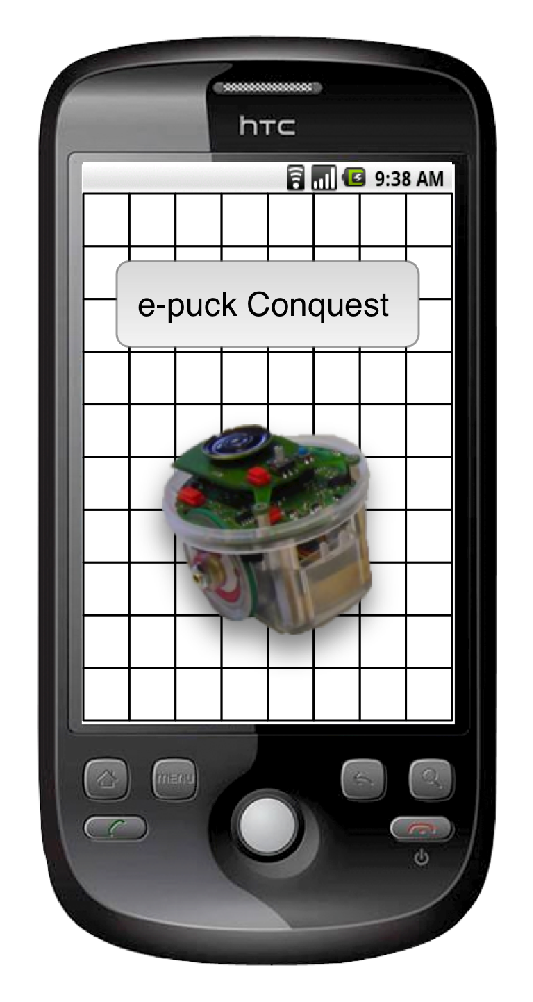
\includegraphics[height=10cm]{logo.eps} \\
	\vspace{1cm}
	Entwurf - epuck Nachrichtensystem
}
\author{Martin Freund}
\begin{document}
	\section{Nachrichtenverarbeitung}
		{Abgesehen von der anfänglichen Initialisierung des Bluetooth-Moduls, verläuft die Übertragung in beide
		Richtungen transparent über den primären UART des e-pucks mit der {\tt hal\_uart1} Schicht. Jeder e-puck besitzt
		sowohl einen Eingangs- als auch	einen Ausgangsringpuffer über welche die Nachrichten von der Hardware empfangen
		bzw. gesendet werden. Die Logik des e-pucks verwendet lediglich die {\tt com}-Schicht um Nachrichten zu
		empfangen bzw. zu senden. Dazu wird der Eingangspuffer von der Logik überwacht. Sobald mindestens eine Nachricht
		vorhanden ist, wird diese über die	{\tt com}-Schicht ausgelesen und an den von der Logik festgelegten Callback
		übergeben.

		Jede e-puck Antwortnachricht hat eine vorhergehende Android Anfragenachricht als Ursache.}
	\section{Nachrichtenformat}
		\begin{itemize}
			\item Jede Nachricht besteht aus 32 Bytes
			\item Das Zahlenformat ist Little-Endian
			\item Die ersten beiden Bytes identifizieren den Nachrichtentyp eindeutig
			\item Die verbleibenden 30 Bytes können nachrichtenspezifisch verwendet werden
		\end{itemize}
	\section{Nachrichtensequenzen}	
		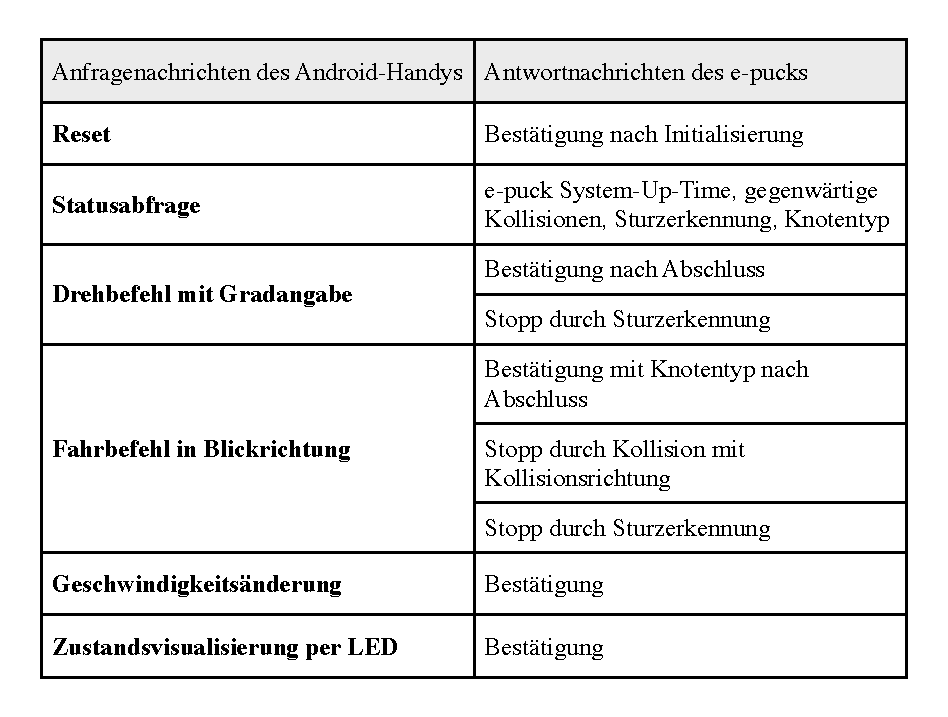
\includegraphics[height=10cm]{images/epuck_bt_msgs.eps}
\end{document}